%! Author = Philipp Emmenegger
%! Date = 09/06/2021

\section{Processes 2}
\subsection{Traditional vs. Agile Planning}
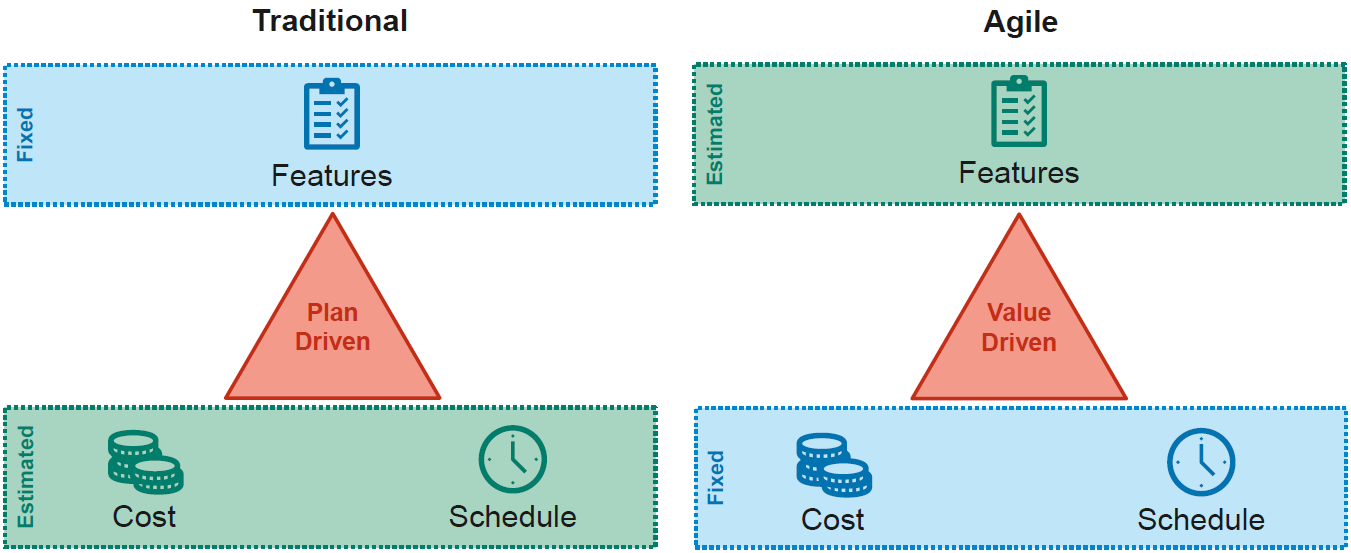
\includegraphics[width=\linewidth]{../img/traditional_vs_agile_planning.png}
\textbf{Common PM work}
\begin{itemize}
    \item Time Tracking
    \item Cost Analysis
    \item Progress Monitoring
    \item Risk Management
    \item Negotiation
    \item Sending invoices
    \item Reporting to management
    \item \textbf{Not managed by Scrum!}
\end{itemize}
\subsubsection{Add a PM role}
\begin{itemize}
    \item Define the role Project Manager
    \item Define responsibilities
    \item Use Sprint Retrospective to reflect them
    \item Smaller projects: assign it to existing members
    \item Larger projects: dedicated person
\end{itemize}

\subsubsection{Making the invisible visible}
\begin{itemize}
    \item Scrum Board
    \item Burndown Charts
    \item Velocity Charts
    \item Git Activity
    \item Build Status
    \item Test Status
    \item Code Metrics
    \item Analytics and Diagnostics
    \item Installations and User Rating
\end{itemize}
\textbf{Dashboards}
\begin{itemize}
    \item Help to understand the progress of the project
    \item Understandable for non-technical users
    \item Not only for the PM, also for the team
    \item Trends over plain numbers
\end{itemize}

\subsection{Scaling Scrum}
\begin{itemize}
    \item Scrum + RUP (Scrum+)
    \item Self made scaling
\end{itemize}

\subsubsection{Self-made scaling}
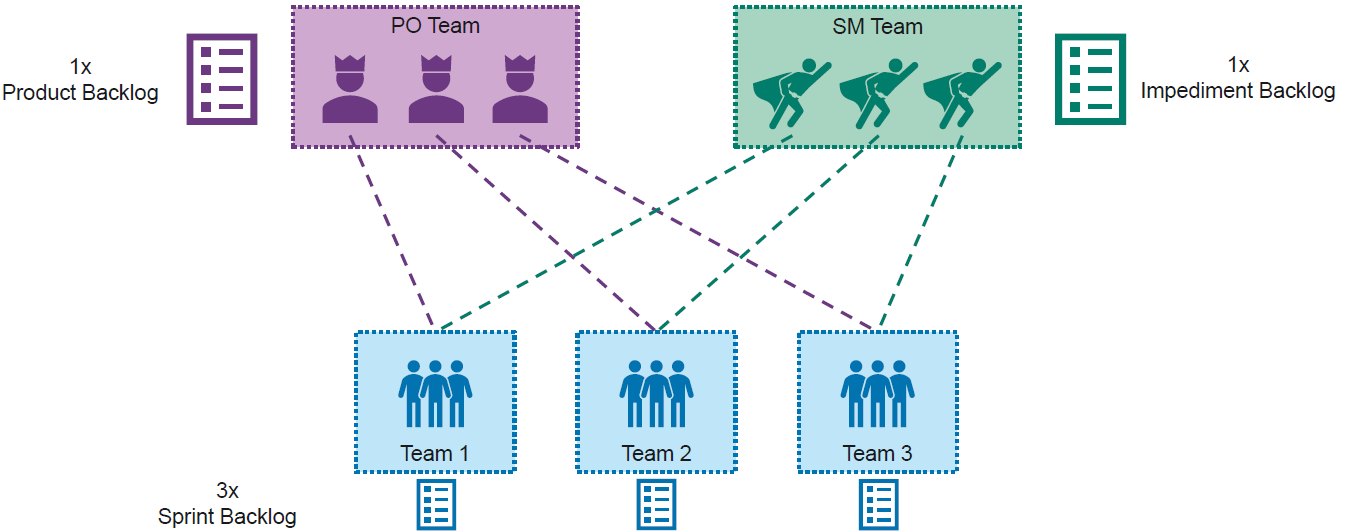
\includegraphics[width=\linewidth]{../img/self_made_scaling.png}
\textbf{Sprint Planning}
\begin{itemize}
    \item Single planning for all teams
    \item Teams allocate stories on their own
    \item Allocation often based on previous refinements
\end{itemize}
\textbf{Daily Scrum}
\begin{itemize}
    \item Separate meeting for every team
    \item Do Scrum of Scrums in addition
\end{itemize}
\textbf{Sprint Review}
\begin{itemize}
    \item Single meeting for all teams
    \item Probably needs a higher level moderator
\end{itemize}
\textbf{Sprint Retrospective}
\begin{itemize}
    \item Single meeting for all teams
    \item All 3-4 sprints also do a Project Retrospective
\end{itemize}

\subsection{Kanban}
\textbf{Principles}
\begin{enumerate}
    \item Start with what you know
    \item Agree to pursue incremental, evolutionary change
    \item Respect the current process, roles, responsibilities \& titles
    \item Encourage acts of leadership at all levels
\end{enumerate}
\textbf{Practices}
\begin{itemize}
    \item Visualize
    \item Limit WIP
    \item Manage Flow
    \item Mage Process Explicit
    \item Implement Feedback Loops
    \item Improve Collaboratively, evolve experimentally
\end{itemize}

\subsubsection{Scrum vs. Kanban}
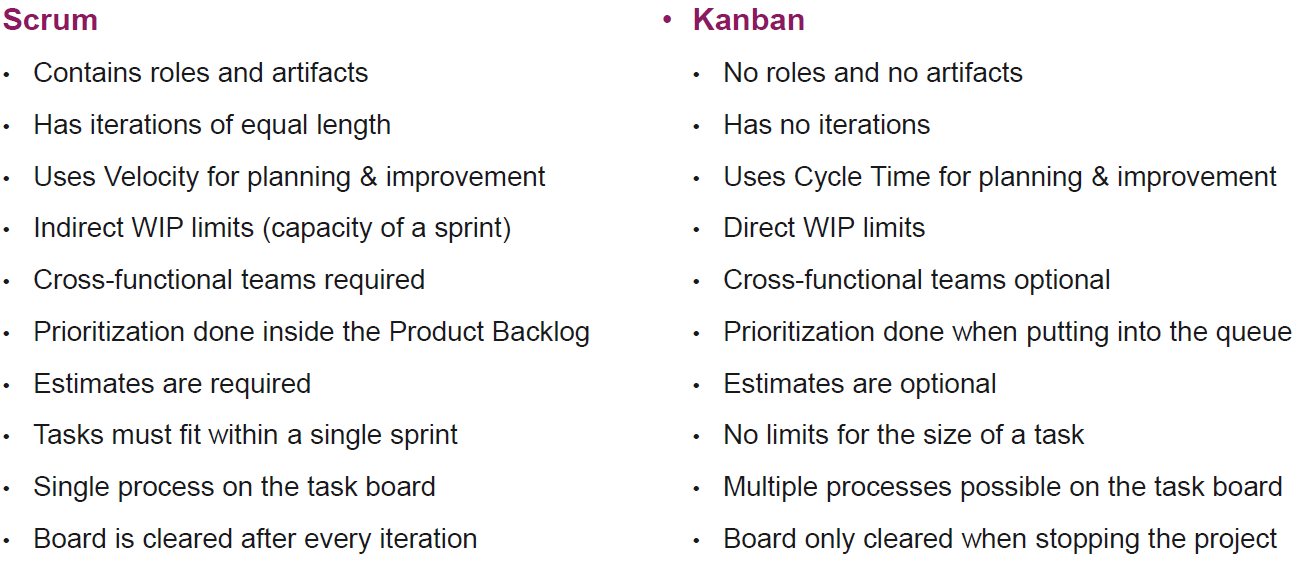
\includegraphics[width=\linewidth]{../img/scrum_vs_kanban.png}